\documentclass{article}
\usepackage{spconf,amsmath,graphicx,subfigure,multirow, bigstrut, paralist}

\usepackage[breaklinks=true,colorlinks,bookmarks=false]{hyperref}

\newcommand{\todo}[1]{\textcolor{red}{todo: {\em #1}}}
\newcommand{\figref}[1]{Figure~\ref{fig:#1}}
\newcommand{\tblref}[1]{Table~\ref{tbl:#1}}

\title{Deep Methods for Estimating Transient Scene Properties}


\name{Ryan Baltenberger, Connor Greenwell, Scott Workman, Nathan Jacobs
  \vspace{-.75em}}
\address{ 
  Department of Computer Science, University of Kentucky \\
  {\tt\small \{rbalten, connor, scott, jacobs\}@cs.uky.edu}
}


\begin{document}

\maketitle

\begin{abstract}

We propose to use deep convolutional neural networks to estimate the
transient attributes of a scene from a single image. Such networks
have been used to achieve state-of-the-art results for many 
vision problems, from object detection to scene classification, but
have not been used for such attributes. Transient scene attributes
describe both the objective conditions, such as the weather, time of
day, and the season, and subjective properties, such whether or not
the scene is busy, of a scene. We compare several methods for
pre-training an existing network architecture and obtain
state-of-the-art results on two benchmark datasets.  We also show how
such networks may be used in several different applications.

\end{abstract}

\begin{keywords}
image understanding, neural networks
\end{keywords}

\section{Introduction}

% general intro to the problem and why it is important

Outdoor scenes experience a wide range of lighting and weather
conditions which dramatically affect their appearance. A scene can
change from rainy and brooding to sunny and pleasant in a matter of
hours, even minutes. The ability to quickly understand these fleeting,
or transient, attributes is a critical skill that people often take
for granted. The ability to automatically understand such subtle
conditions has many potential application, including: improving
context-dependent anomaly detection~\cite{abrams12lost}; enabling
attribute-oriented browsing and search of large image
sets\cite{jacobs07amos,skyfinder}; estimating micro-climate conditions
using outdoor webcams~\cite{islam13webcamweather}; as a pre-processing
step for higher-level algorithms for
calibration~\cite{jacobs13cloudcalibration,workman2014rainbow}, shape
estimation~\cite{heliometric,abramsheliometric},
geolocalization~\cite{jacobs07geolocate}; and  environmental
monitoring~\cite{jacobs09webcamgis}. 

% what do we propose to do? 

We propose a method for predicting transient attributes from a single
image using deep convolutional neural networks. Such techniques have
has been used to obtain state-of-the-art results in problems ranging
from object classification~\cite{krizhevsky2012imagenet}, object
detection~\cite{girshick2013rich}, and scene
classification~\cite{zhou2014places} but have not been used to
estimate transient scene attributes. We address two problems in
estimating transient scene attributes. One is the problem of
estimating whether it is sunny or cloudy~\cite{lutwoclass} and the
other is predicting the degree to which various transient attributes
are present in the scene~\cite{Laffont14}. We consider 2 different
networks and 3 different training methods.

\begin{figure}
	\centering
		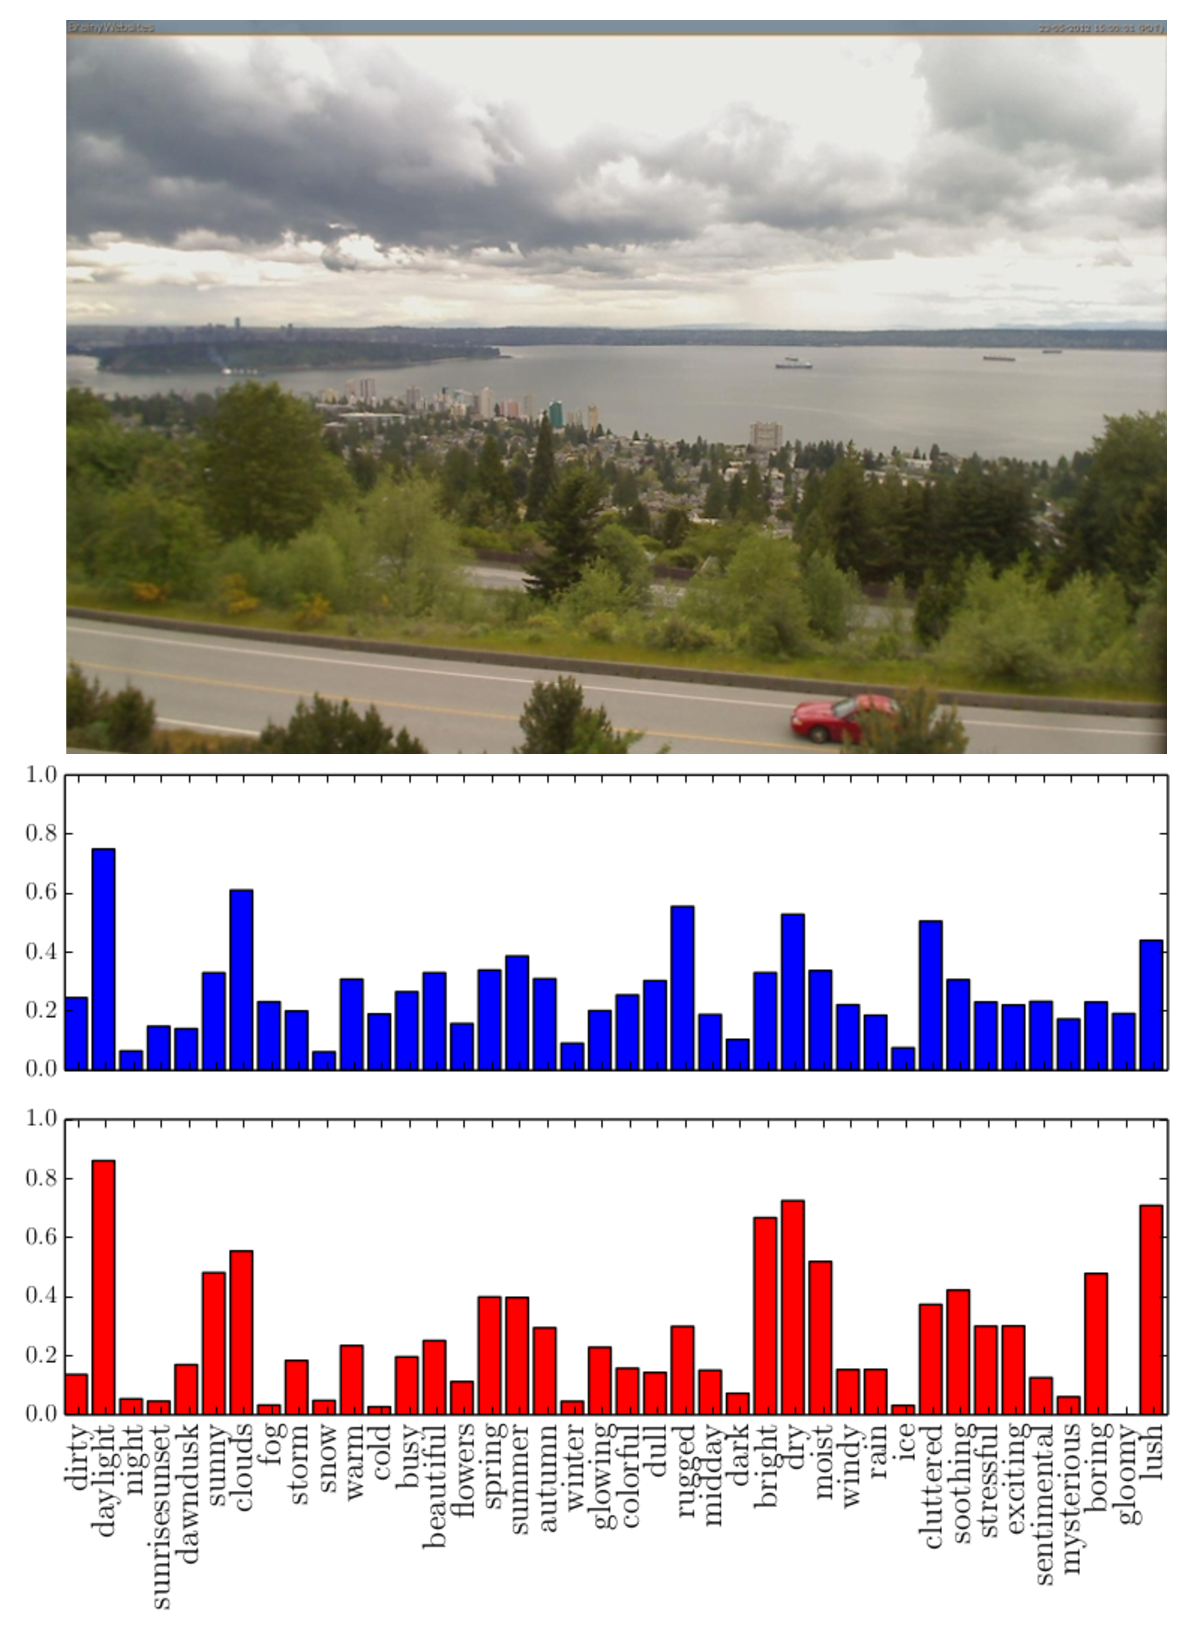
\includegraphics[width=0.5\textwidth]{figs/bars.pdf}
		\caption{Example images from the Transient Attributes Dataset
      with our network's confidence in each predicted label.}
    \label{fig:results}
\end{figure}

% what we can do now that we have this?

The key contributions of this work are: 1) a comparison of several
deep learning network training methods for predicting transient
attributes, 2) an evaluation on two benchmark
datasets~\cite{lutwoclass,Laffont14}, which shows the proposed
networks achieve state-of-the-art performance, and 3) releasing six
pre-trained networks for classifying transient scene attributes
publicly available in a popular deep learning
framework~\cite{caffe14}. 

\subsection{Related Work}

Visual attributes are high-level descriptions of a visual property
which offer some additional semantic context for understanding an
object, activity, or scene. For example, a \emph{green} apple or a
\emph{cloudy} day. Representations based on such visual attributes
have become increasingly popular in the vision community as they offer
the ability to to generalize across categories. The first
learning-based methods to take advantage of such high-level attributes
arose for the task of object
recognition~\cite{farhadi2009describing,lampert2009learning},
demonstrating the power of learning by description. Many methods were
quick to follow suit, with applications ranging from content-based
image retrieval~\cite{siddiquie2011image} to characterizing facial
appearance~\cite{kumar2011describable}. Given their prowess, a
significant amount of research has focused on identifying useful
attributes~\cite{berg2010automatic} and crafting techniques to
accurately detect them in images~\cite{vedaldi2014understanding}. 

More recently, efforts have been made to adapt such attribute-based
representations for outdoor scene understanding, where the appearance
of a scene can change drastically over time.  Patterson and
Hays~\cite{patterson2012sun} constructed the SUN attribute dataset
using crowd-sourcing techniques to identify a taxonomy of 102 scene
attributes from human descriptions, designed to distinguish between
scene categories. Similarly, Laffont et al.~\cite{Laffont14} introduce the
Transient Attributes dataset, focused instead on perceived scene
properties and attributes that describe intra-scene variations. They
define 40 such attributes, and present methods for identifying the
presence of those attributes as well as applications in photo
organization and high-level image editing via attribute manipulation. 

To the best of our knowledge, we are the first to explore the
application of deep learning architectures for learning such
attributes using only the raw image intensities as input.

\subsection{Background}

Deep convolutional neural networks (CNNs) have been used extensively
in recent years to obtain state-of-the-art results on a wide variety
of computer vision problems.  In this work, we focus on a particular
CNN architecture, often called ``AlexNet'', introduced by Alex
Krizhevsky et al.~\cite{caffenetnips12} for single-image object
classification. This network has eight layers with trainable
parameters: five convolutional layers (each connected, in a
feed-forward manner with pooling and dropout layers between each
convolutional layer) and three fully connected layers. Essentially,
the convolutional layers extract features from across the image and
the fully connected layers combine these features to obtain a score
for each possible class. The final classification decision is obtained
by choosing the class with the highest output score.

While this network architecture was originally developed for
single-image object classification, it has been shown to be adaptable
to other problem domains. If the new problem involves multi-class
classification, all that is needed is to modify the final fully
connected layer to have the correct number of output classes. Then the
network weights can be `fine-tuned' by running iterations of stochastic
gradient descent on the training data for the new problem.  The key is
to start the optimization with random weights for the new final layer
and weights from an already trained network, for example using the
weights from the original AlexNet~\cite{caffenetnips12}, as an initial
condition. This approach was overviewed
in~\cite{yosinski2014transferable}. If there is a large amount of
training data available for the new domain, it is also possible to
train the network from scratch by randomly initializing all
weights~\cite{zhou2014places}.  If the new problem domain is
regression, not classification, then the only change that is necessary
is to change the network loss function, perhaps replacing the SOFT-MAX
loss with an $L_2$ loss.

\section{Deep Networks for Estimating Transient Attributes}

We propose to use deep convolutional neural networks to classify
transient scene attributes. We develop networks for two single-image
problems: the classification problem of estimating whether it is sunny
or cloudy (CloudyNet) and a collection of regression problems that
represent the degree to which a large number of transient attribute
describe the scene (TransientNet).  For each of these problems, we
use three different networks as starting conditions for optimization,
resulting in a total of six networks.  For both problems, we use the
``AlexNet'' CNN architecture, described in the previous section.  The
remainder of this section describes how we estimate network weights
for each of these networks.

\begin{figure*}[t!]
	\centering
		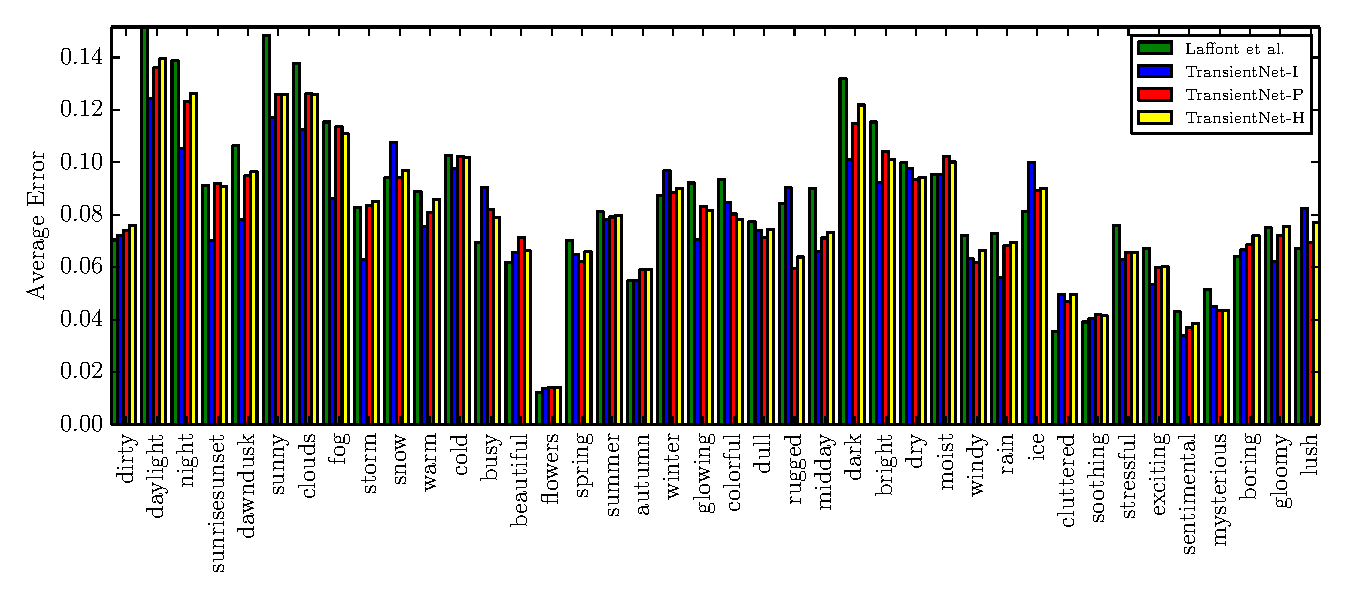
\includegraphics[width=1.0\textwidth]{figs/avg_err_compare_cmr.pdf}
		\caption{This shows the average errors for each attribute from proposed method
						 by Laffont et al., TransientNet-I, TransientNet-P, and TransientNet-H.  
             TransientNet-S has the lowest average error for most of the attributes.}
		\label{fig:compare}
\end{figure*}

\textbf{CloudyNet:} For the problem of classifying whether an image is
sunny or cloudy, we use the data provided by Lu~\cite{lutwoclass} et
al.\ to train our network, which we call CloudyNet.  We follow their
protocol for training and testing: each list of sunny/cloudy images
was randomly shuffled and the first 80\% of each list was chosen as
the training data and the last 20\% was chosen as testing data.  The
only modification to the network architecture that was required was
dropping unnecessary output nodes from the final fully connected layer
(in the end we have two output nodes).

\textbf{TransientNet:} In addition, we train a network for the more
challenging problem of estimating a broad range of attributes proposed
by Laffont~\cite{Laffont14}.  In this problem, there are 40 transient
attributes (see \figref{compare} for the full list of
attributes), each of which is assigned a value between zero and one
for an image. We use the training set defined by
Laffont~\cite{Laffont14} in which the images from 81 webcams are used
for training and images from a distinct set of 20 webcams is used for
testing.  The only modification of the network architecture that was
required was changing the final fully connected layer to have 40
nodes, one for each transient attribute, and changing the loss
function to a Euclidean loss. 

We trained both of these networks using three different initial
conditions resulting in six distinct sets of network weights. The
first set of initial conditions are taken from a network that was was
trained for scene classification on 1.2 million images from the
ImageNet ILSVRC-2012 challenge~\cite{ILSVRCarxiv14}.  We call the
networks that result from this fine-tuning process CloudyNet-I and
TransientNet-I.  The second set of initial conditions were taken from
a network~\cite{zhou2014places} was trained for scene classification
on 2.5 million images with labels in 205 categories from the Places
Database~\cite{zhou2014places}. We call the resulting networks
CloudyNet-P and TransientNet-P.  The final set of initial conditions
were taken from a network that was trained~\cite{zhou2014places} for
both object and scene classification.  This hybrid network was trained
on a combination of the Places Database~\cite{zhou2014places} and
images from the training data of ILSVRC-2012
challenge~\cite{ILSVRCarxiv14}.  The full training set contained 205
scene categories from the Places Database and 978 object categories
from ILSVRC-2012 totaling about 3.6 million images.  We call the
resulting networks CloudyNet-H and TransientNet-H.

\textbf{Implementation Details:} We train each networks using the
Caffe~\cite{caffe14} deep learning software framework, the Caffenet
reference network architecture, and pre-trained networks from the
Caffe Model
Zoo\footnote{\url{http://caffe.berkeleyvision.org/model_zoo.html}}.
All of our networks were trained on NVIDIA M2075 GPU Cards for 24 hours
each, and evaluated using Caffe in CPU mode on Dell C6220 Servers 
equipped with Dual Intel E5-2670 8 Core (Sandy Bridge) @ 2.6 GHz.
The full network
optimization definition, the final network weights, and the output
from our methods will be made available online for all six networks.

\section{Evaluation}

We evaluate the six networks defined in the previous section on two
large-scale benchmark datasets. The results show that these deep
networks obtain state-of-the-the-art results. 

\subsection{Two-Class Weather Classification}

In our first experiment, we use the dataset created by Lu et al.~\cite{lutwoclass} to train
our networks for two class weather classification.  The dataset
contains images collected from the SUN Database~\cite{xiaoSUN}, the
LabelMe Database~\cite{russell2008labelme}, and Flickr. The dataset
contains 5000 sunny and 5000 cloudy images. Flickr images were
collected manually by ``helpers'' unaware of the purpose or methods of
Lu et al. The dataset was then pruned for images with similar
histograms, and finally pruned by another round of helpers to narrow
the dataset to 10,000 images.  \tblref{twoclass} shows the normalized
accuracies of our networks compared to the method proposed by
Lu et al~\cite{lutwoclass}.  The normalized accuracy was calculated by
$ \max\{((a - 0.5) / 0.5), 0\} $, where $a$ is the traditionally
obtained accuracy. All three of the networks outperform the state of
the art for two class weather classification with CloudyNet-P
predicting the most accurately.  CloudyNet-P averages 0.0672s per
image for prediction. 

\subsection{Transient Attributes}

We used the dataset created by Laffont et al.~\cite{Laffont14} to
train our networks for transient attribute prediction. The dataset
contains images from outdoor webcams in the Archive of Many Outdoor
Scenes~\cite{jacobs07amos} and the Webcam Clip Art
Dataset~\cite{lalondesig09}.  The webcams span a wide range of outdoor
scenes, from urban regions to wooded, mountainous regions. Each webcam
has 60-120 representative images that feature variations in weather,
lighting conditions, etc.  The images are high resolution and are
aligned to a reference frame through a homography warp with manually
specified correspondences.  The final dataset consists of 8571 images
from 101 webcams.

\figref{compare} shows the average errors from TransientNet-I, TransientNet-P, 
TransientNet-H and Laffont et al. for each attribute in the dataset.  TransientNet-I 
performs best on more than half of the attributes and is the best performing CNN that we trained.  
Transient has the lowest overall average error as shown in \tblref{transient}.  TransientNet-P
and TransientNet-H have similar performance, mostly due to them being pretrained on similar 
sets of data.

\figref{relerr} shows the relative error between our method using TransientNet-I
and the method presented in~\cite{Laffont14}.  The average relative error 
for each attribute using the method in~\cite{Laffont14} was subtracted from
the average relative error using TransientNet-I.  A negative value means TransientNet-I
had a smaller error and a positive value means~\cite{Laffont14} had a smaller
error.  For example, the difference between the two methods on the attribute
night was around 3.2 percentage points, with TransientNet-I having the smaller 
error.  TransientNet-I averages 0.0699s per image for prediction. 

\begin{table}[t]
	\centering
	\begin{tabular}{ | l | c | }
		\hline
			Method & Normalized Accuracy \\ \hline
			Lu et al.~\cite{lutwoclass}& 53.1\% \\ \hline
			CloudyNet-I & 81.8\% \\ \hline
			CloudyNet-P & \textbf{84.7\%} \\ \hline
			CloudyNet-H & 83.1\% \\ 
		\hline
	\end{tabular}
	\caption{Two Class Weather Classification Accuracy}
	\label{tbl:twoclass}
\end{table}

\begin{table}
  \renewcommand{\arraystretch}{2}
  \centering
  \begin{tabular}[b]{| c | c |}
    \hline
    Image & Labels \\
    \hline
    \multirow{3}[3]{*}[-2mm]{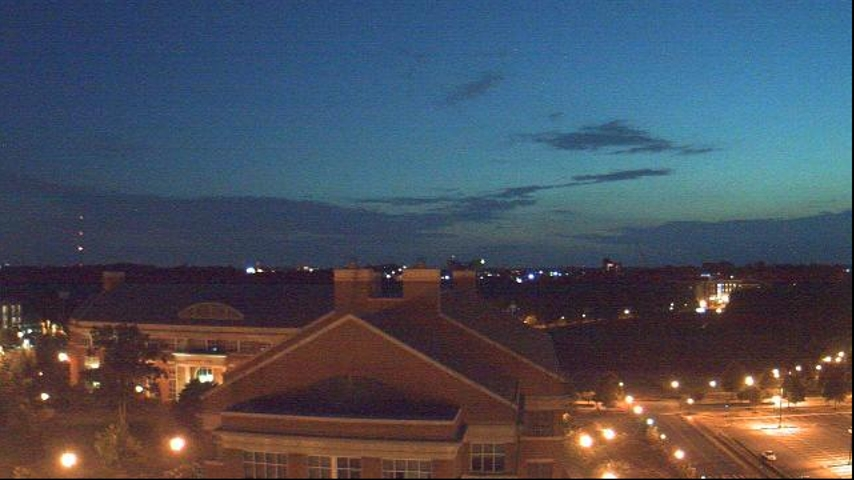
\includegraphics[width=0.19\textwidth]{figs/labels_1.jpg}}
      & night, not sunny \bigstrut \\
      & dark, not snow \bigstrut  \\
      & glowing, not midday \bigstrut  \\
    \hline
    \multirow{3}[3]{*}[-2mm]{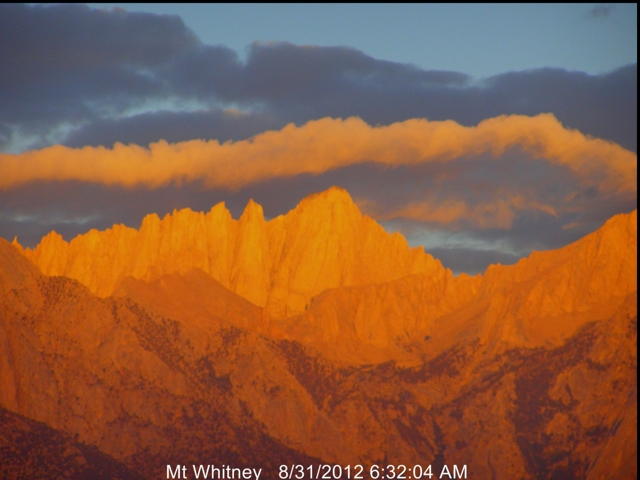
\includegraphics[width=0.18\textwidth]{figs/labels_2.jpg}}
      & rugged, not flowers \bigstrut  \\
      & dawndusk, not rain \bigstrut  \\
      & sunrisesunset, not storm  \bigstrut \\
    \hline
  \end{tabular}
  \caption{example labels}
  \label{tbl:labels}
\end{table}

\begin{figure}[t]
	\centering
		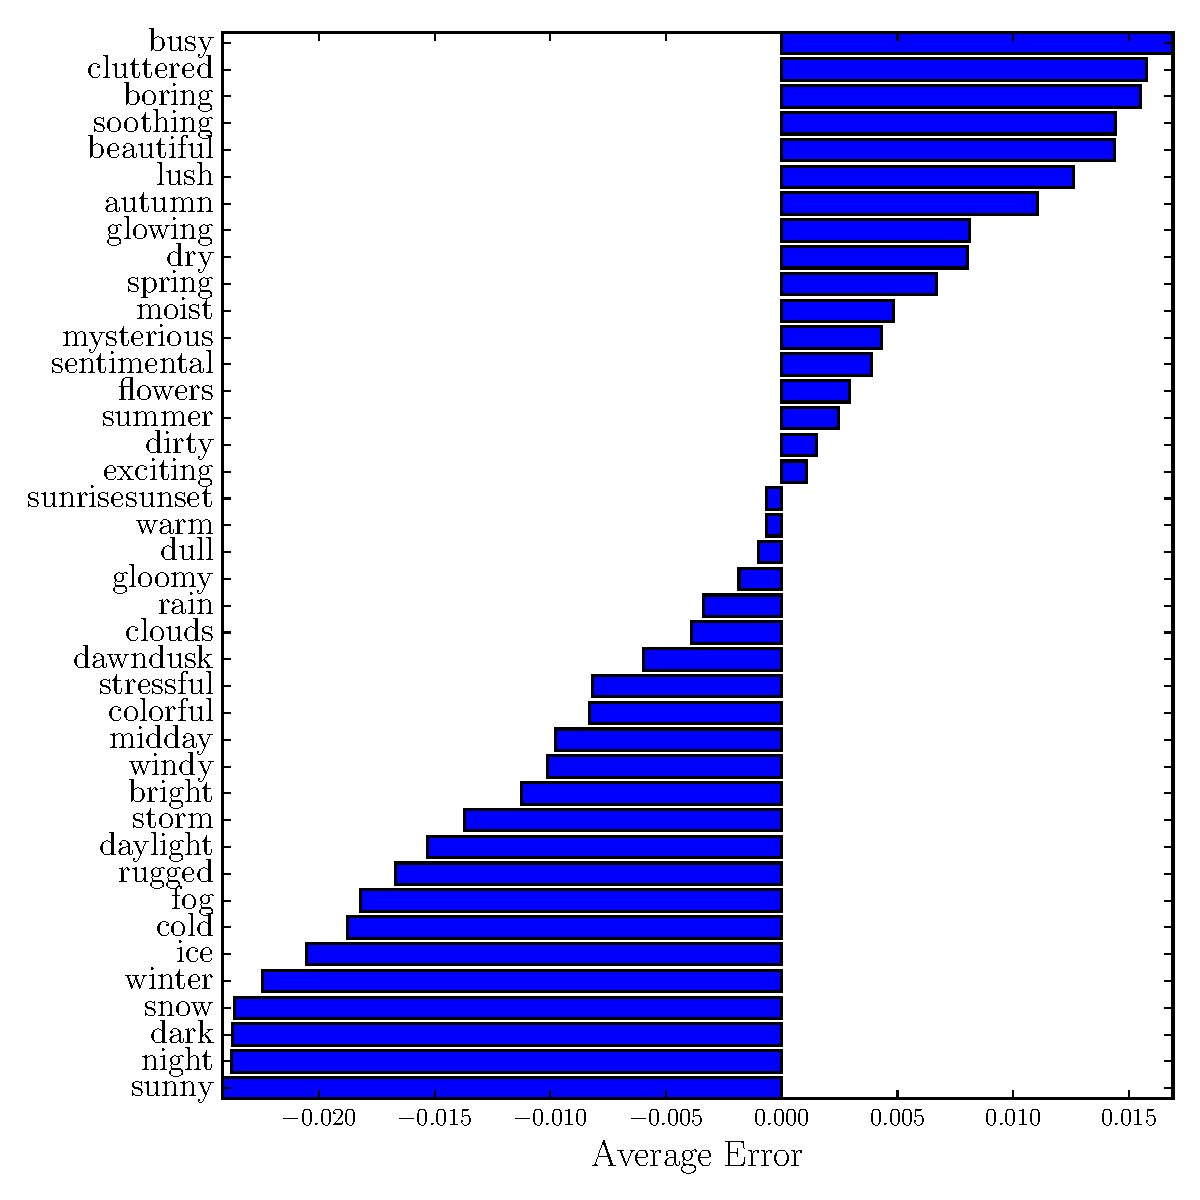
\includegraphics[width=0.5\textwidth]{figs/rel_err_cmr.pdf}
		\caption{This shows the relative errors of TransientNet-I against the method 
						 proposed by Laffont et al. for each attribute.  Attributes with a 
						 negative average error are attributes that are predicting more 
						 accurately by our method.}
		\label{fig:relerr}
\end{figure}

\begin{table}[t]
	\centering
	\begin{tabular}{ | l | c | }
		\hline
			Method & Average Error \\ \hline
			Laffont et al.~\cite{Laffont14}& 8.48\% \\ \hline
			TransientNet-I & \textbf{7.65\%} \\ \hline
			TransientNet-P & 8.02\% \\ \hline
			TransientNet-H & 8.13\% \\ 
		\hline
	\end{tabular}
	\caption{Transient Attribute prediction errors}
	\label{tbl:transient}
\end{table}

\section{Applications}
\subsection{Automatic Webcam Image Labeling}
\indent

One application of transient attribute estimation is automatic outdoor
webcam labeling. Webcam collections such as AMOS\cite{jacobs07amos} contain
thousands of geolocated webcams with years of archived data.  Searching
for an scenes with a set of desired attributes is usually done by manually
looking through lists of webcams and images.  TransientNet can simplify this
process by using the output scores to tag images and webcams with certain 
attributes.  If an attribute is above a defined threshold, the image could 
be labeled with that attribute.  The opposite could be true as well.  If an
attribute is below a defined threshold, the attribute could be added to a 
list of attributes the image does not have.  \tblref{labels} shows examples of
the potential labels for images. This would enable users to use queries such 
as "sunny" or "not winter".  Attributes that appear frequently in a webcam 
(aside from daylight, night, etc) could be used to tag the webcam.  This would 
allow for much easier searching of large collections of webcams.

\section{Conclusions}

We introduce six deep convolutional neural networks for predicting
transient scene attributes from a single image. These networks achieve
state-of-the-art results on two benchmark datasets. The key advantages
of the proposed approach are that it requires no hand-engineered
features, is simple to train, is very fast at test time, and makes
accurate predictions. In addition, these networks can quickly extended
to label additional attributes or adapted to new datasets with a small
amount of retraining. In future work, we plan to explore the use of
these networks in an application to micro-climate estimation from
publicly available outdoor webcams~\cite{islam13webcamweather}. 

{\small
\bibliographystyle{IEEEbib}
\bibliography{refs}
}

\end{document}
